
%% bare_conf.tex
%% V1.3
%% 2007/01/11
%% by Michael Shell
%% See:
%% http://www.michaelshell.org/
%% for current contact information.
%%
%% This is a skeleton file demonstrating the use of IEEEtran.cls
%% (requires IEEEtran.cls version 1.7 or later) with an IEEE conference paper.
%%
%% Support sites:
%% http://www.michaelshell.org/tex/ieeetran/
%% http://www.ctan.org/tex-archive/macros/latex/contrib/IEEEtran/
%% and
%% http://www.ieee.org/

%%*************************************************************************
%% Legal Notice:
%% This code is offered as-is without any warranty either expressed or
%% implied; without even the implied warranty of MERCHANTABILITY or
%% FITNESS FOR A PARTICULAR PURPOSE! 
%% User assumes all risk.
%% In no event shall IEEE or any contributor to this code be liable for
%% any damages or losses, including, but not limited to, incidental,
%% consequential, or any other damages, resulting from the use or misuse
%% of any information contained here.
%%
%% All comments are the opinions of their respective authors and are not
%% necessarily endorsed by the IEEE.
%%
%% This work is distributed under the LaTeX Project Public License (LPPL)
%% ( http://www.latex-project.org/ ) version 1.3, and may be freely used,
%% distributed and modified. A copy of the LPPL, version 1.3, is included
%% in the base LaTeX documentation of all distributions of LaTeX released
%% 2003/12/01 or later.
%% Retain all contribution notices and credits.
%% ** Modified files should be clearly indicated as such, including  **
%% ** renaming them and changing author support contact information. **
%%
%% File list of work: IEEEtran.cls, IEEEtran_HOWTO.pdf, bare_adv.tex,
%%                    bare_conf.tex, bare_jrnl.tex, bare_jrnl_compsoc.tex
%%*************************************************************************

% *** Authors should verify (and, if needed, correct) their LaTeX system  ***
% *** with the testflow diagnostic prior to trusting their LaTeX platform ***
% *** with production work. IEEE's font choices can trigger bugs that do  ***
% *** not appear when using other class files.                            ***
% The testflow support page is at:
% http://www.michaelshell.org/tex/testflow/



% Note that the a4paper option is mainly intended so that authors in
% countries using A4 can easily print to A4 and see how their papers will
% look in print - the typesetting of the document will not typically be
% affected with changes in paper size (but the bottom and side margins will).
% Use the testflow package mentioned above to verify correct handling of
% both paper sizes by the user's LaTeX system.
%
% Also note that the "draftcls" or "draftclsnofoot", not "draft", option
% should be used if it is desired that the figures are to be displayed in
% draft mode.
%
\documentclass[conference]{IEEEtran}
% Add the compsoc option for Computer Society conferences.
%
% If IEEEtran.cls has not been installed into the LaTeX system files,
% manually specify the path to it like:
% \documentclass[conference]{../sty/IEEEtran}


\usepackage[francais,english]{babel}
\usepackage{aeguill}
\usepackage[utf8]{inputenc}
\usepackage[T1]{fontenc}
%\usepackage[latin1]{inputenc} %% For ISO-latin1 chars
                                %% (accented letters).
\usepackage{txfonts}



% Some very useful LaTeX packages include:
% (uncomment the ones you want to load)


% *** MISC UTILITY PACKAGES ***
%
%\usepackage{ifpdf}
% Heiko Oberdiek's ifpdf.sty is very useful if you need conditional
% compilation based on whether the output is pdf or dvi.
% usage:
% \ifpdf
%   % pdf code
% \else
%   % dvi code
% \fi
% The latest version of ifpdf.sty can be obtained from:
% http://www.ctan.org/tex-archive/macros/latex/contrib/oberdiek/
% Also, note that IEEEtran.cls V1.7 and later provides a builtin
% \ifCLASSINFOpdf conditional that works the same way.
% When switching from latex to pdflatex and vice-versa, the compiler may
% have to be run twice to clear warning/error messages.






% *** CITATION PACKAGES ***
%
%\usepackage{cite}
% cite.sty was written by Donald Arseneau
% V1.6 and later of IEEEtran pre-defines the format of the cite.sty package
% \cite{} output to follow that of IEEE. Loading the cite package will
% result in citation numbers being automatically sorted and properly
% "compressed/ranged". e.g., [1], [9], [2], [7], [5], [6] without using
% cite.sty will become [1], [2], [5]--[7], [9] using cite.sty. cite.sty's
% \cite will automatically add leading space, if needed. Use cite.sty's
% noadjust option (cite.sty V3.8 and later) if you want to turn this off.
% cite.sty is already installed on most LaTeX systems. Be sure and use
% version 4.0 (2003-05-27) and later if using hyperref.sty. cite.sty does
% not currently provide for hyperlinked citations.
% The latest version can be obtained at:
% http://www.ctan.org/tex-archive/macros/latex/contrib/cite/
% The documentation is contained in the cite.sty file itself.






% *** GRAPHICS RELATED PACKAGES ***
%
\ifCLASSINFOpdf
   \usepackage[pdftex]{graphicx}
  % declare the path(s) where your graphic files are
  % \graphicspath{{../pdf/}{../jpeg/}}
  % and their extensions so you won't have to specify these with
  % every instance of \includegraphics
  % \DeclareGraphicsExtensions{.pdf,.jpeg,.png}
\else
  % or other class option (dvipsone, dvipdf, if not using dvips). graphicx
  % will default to the driver specified in the system graphics.cfg if no
  % driver is specified.
  % \usepackage[dvips]{graphicx}
  % declare the path(s) where your graphic files are
  % \graphicspath{{../eps/}}
  % and their extensions so you won't have to specify these with
  % every instance of \includegraphics
  % \DeclareGraphicsExtensions{.eps}
\fi
% graphicx was written by David Carlisle and Sebastian Rahtz. It is
% required if you want graphics, photos, etc. graphicx.sty is already
% installed on most LaTeX systems. The latest version and documentation can
% be obtained at: 
% http://www.ctan.org/tex-archive/macros/latex/required/graphics/
% Another good source of documentation is "Using Imported Graphics in
% LaTeX2e" by Keith Reckdahl which can be found as epslatex.ps or
% epslatex.pdf at: http://www.ctan.org/tex-archive/info/
%
% latex, and pdflatex in dvi mode, support graphics in encapsulated
% postscript (.eps) format. pdflatex in pdf mode supports graphics
% in .pdf, .jpeg, .png and .mps (metapost) formats. Users should ensure
% that all non-photo figures use a vector format (.eps, .pdf, .mps) and
% not a bitmapped formats (.jpeg, .png). IEEE frowns on bitmapped formats
% which can result in "jaggedy"/blurry rendering of lines and letters as
% well as large increases in file sizes.
%
% You can find documentation about the pdfTeX application at:
% http://www.tug.org/applications/pdftex





% *** MATH PACKAGES ***
%
%\usepackage[cmex10]{amsmath}
% A popular package from the American Mathematical Society that provides
% many useful and powerful commands for dealing with mathematics. If using
% it, be sure to load this package with the cmex10 option to ensure that
% only type 1 fonts will utilized at all point sizes. Without this option,
% it is possible that some math symbols, particularly those within
% footnotes, will be rendered in bitmap form which will result in a
% document that can not be IEEE Xplore compliant!
%
% Also, note that the amsmath package sets \interdisplaylinepenalty to 10000
% thus preventing page breaks from occurring within multiline equations. Use:
%\interdisplaylinepenalty=2500
% after loading amsmath to restore such page breaks as IEEEtran.cls normally
% does. amsmath.sty is already installed on most LaTeX systems. The latest
% version and documentation can be obtained at:
% http://www.ctan.org/tex-archive/macros/latex/required/amslatex/math/





% *** SPECIALIZED LIST PACKAGES ***
%
%\usepackage{algorithmic}
% algorithmic.sty was written by Peter Williams and Rogerio Brito.
% This package provides an algorithmic environment fo describing algorithms.
% You can use the algorithmic environment in-text or within a figure
% environment to provide for a floating algorithm. Do NOT use the algorithm
% floating environment provided by algorithm.sty (by the same authors) or
% algorithm2e.sty (by Christophe Fiorio) as IEEE does not use dedicated
% algorithm float types and packages that provide these will not provide
% correct IEEE style captions. The latest version and documentation of
% algorithmic.sty can be obtained at:
% http://www.ctan.org/tex-archive/macros/latex/contrib/algorithms/
% There is also a support site at:
% http://algorithms.berlios.de/index.html
% Also of interest may be the (relatively newer and more customizable)
% algorithmicx.sty package by Szasz Janos:
% http://www.ctan.org/tex-archive/macros/latex/contrib/algorithmicx/




% *** ALIGNMENT PACKAGES ***
%
%\usepackage{array}
% Frank Mittelbach's and David Carlisle's array.sty patches and improves
% the standard LaTeX2e array and tabular environments to provide better
% appearance and additional user controls. As the default LaTeX2e table
% generation code is lacking to the point of almost being broken with
% respect to the quality of the end results, all users are strongly
% advised to use an enhanced (at the very least that provided by array.sty)
% set of table tools. array.sty is already installed on most systems. The
% latest version and documentation can be obtained at:
% http://www.ctan.org/tex-archive/macros/latex/required/tools/


%\usepackage{mdwmath}
%\usepackage{mdwtab}
% Also highly recommended is Mark Wooding's extremely powerful MDW tools,
% especially mdwmath.sty and mdwtab.sty which are used to format equations
% and tables, respectively. The MDWtools set is already installed on most
% LaTeX systems. The lastest version and documentation is available at:
% http://www.ctan.org/tex-archive/macros/latex/contrib/mdwtools/


% IEEEtran contains the IEEEeqnarray family of commands that can be used to
% generate multiline equations as well as matrices, tables, etc., of high
% quality.


%\usepackage{eqparbox}
% Also of notable interest is Scott Pakin's eqparbox package for creating
% (automatically sized) equal width boxes - aka "natural width parboxes".
% Available at:
% http://www.ctan.org/tex-archive/macros/latex/contrib/eqparbox/





% *** SUBFIGURE PACKAGES ***
%\usepackage[tight,footnotesize]{subfigure}
% subfigure.sty was written by Steven Douglas Cochran. This package makes it
% easy to put subfigures in your figures. e.g., "Figure 1a and 1b". For IEEE
% work, it is a good idea to load it with the tight package option to reduce
% the amount of white space around the subfigures. subfigure.sty is already
% installed on most LaTeX systems. The latest version and documentation can
% be obtained at:
% http://www.ctan.org/tex-archive/obsolete/macros/latex/contrib/subfigure/
% subfigure.sty has been superceeded by subfig.sty.



%\usepackage[caption=false]{caption}
%\usepackage[font=footnotesize]{subfig}
% subfig.sty, also written by Steven Douglas Cochran, is the modern
% replacement for subfigure.sty. However, subfig.sty requires and
% automatically loads Axel Sommerfeldt's caption.sty which will override
% IEEEtran.cls handling of captions and this will result in nonIEEE style
% figure/table captions. To prevent this problem, be sure and preload
% caption.sty with its "caption=false" package option. This is will preserve
% IEEEtran.cls handing of captions. Version 1.3 (2005/06/28) and later 
% (recommended due to many improvements over 1.2) of subfig.sty supports
% the caption=false option directly:
%\usepackage[caption=false,font=footnotesize]{subfig}
%
% The latest version and documentation can be obtained at:
% http://www.ctan.org/tex-archive/macros/latex/contrib/subfig/
% The latest version and documentation of caption.sty can be obtained at:
% http://www.ctan.org/tex-archive/macros/latex/contrib/caption/




% *** FLOAT PACKAGES ***
%
%\usepackage{fixltx2e}
% fixltx2e, the successor to the earlier fix2col.sty, was written by
% Frank Mittelbach and David Carlisle. This package corrects a few problems
% in the LaTeX2e kernel, the most notable of which is that in current
% LaTeX2e releases, the ordering of single and double column floats is not
% guaranteed to be preserved. Thus, an unpatched LaTeX2e can allow a
% single column figure to be placed prior to an earlier double column
% figure. The latest version and documentation can be found at:
% http://www.ctan.org/tex-archive/macros/latex/base/



%\usepackage{stfloats}
% stfloats.sty was written by Sigitas Tolusis. This package gives LaTeX2e
% the ability to do double column floats at the bottom of the page as well
% as the top. (e.g., "\begin{figure*}[!b]" is not normally possible in
% LaTeX2e). It also provides a command:
%\fnbelowfloat
% to enable the placement of footnotes below bottom floats (the standard
% LaTeX2e kernel puts them above bottom floats). This is an invasive package
% which rewrites many portions of the LaTeX2e float routines. It may not work
% with other packages that modify the LaTeX2e float routines. The latest
% version and documentation can be obtained at:
% http://www.ctan.org/tex-archive/macros/latex/contrib/sttools/
% Documentation is contained in the stfloats.sty comments as well as in the
% presfull.pdf file. Do not use the stfloats baselinefloat ability as IEEE
% does not allow \baselineskip to stretch. Authors submitting work to the
% IEEE should note that IEEE rarely uses double column equations and
% that authors should try to avoid such use. Do not be tempted to use the
% cuted.sty or midfloat.sty packages (also by Sigitas Tolusis) as IEEE does
% not format its papers in such ways.





% *** PDF, URL AND HYPERLINK PACKAGES ***
%
%\usepackage{url}
% url.sty was written by Donald Arseneau. It provides better support for
% handling and breaking URLs. url.sty is already installed on most LaTeX
% systems. The latest version can be obtained at:
% http://www.ctan.org/tex-archive/macros/latex/contrib/misc/
% Read the url.sty source comments for usage information. Basically,
% \url{my_url_here}.





% *** Do not adjust lengths that control margins, column widths, etc. ***
% *** Do not use packages that alter fonts (such as pslatex).         ***
% There should be no need to do such things with IEEEtran.cls V1.6 and later.
% (Unless specifically asked to do so by the journal or conference you plan
% to submit to, of course. )

% todo macro
\usepackage{color}
\newcommand{\todo}[1]{\noindent\textcolor{red}{{\bf \{ToDo} #1{\bf \}}}}

% correct bad hyphenation here
\hyphenation{op-tical net-works semi-conduc-tor}


\begin{document}
%
% paper title
% can use linebreaks \\ within to get better formatting as desired
\title{Video Recording and Indexing of Theatre Rehearsals}


% author names and affiliations
% use a multiple column layout for up to three different
% affiliations
\author{
\IEEEauthorblockN{Remi Ronfard\\ Vineet Gandhi}
\IEEEauthorblockA{INRIA, LJK\\
University of Grenoble, France\\
Email: remi.ronfard@inria.fr}
\and
\IEEEauthorblockN{Benoit Encelle\\ Pierre-Antoine Champin\\ Thomas Steiner}
\IEEEauthorblockA{Université Claude Bernard\\
Lyon, France\\
Email: xxx}
\and
\IEEEauthorblockN{Nicolas Sauret}
\IEEEauthorblockA{IRI, France\\
Email: nicolas.sauret@iri.centrepompidou.fr}
\and
\IEEEauthorblockN{Cyrille Migniot}
\IEEEauthorblockA{University of Burgundy, France\\
Email: xxx}
}

% conference papers do not typically use \thanks and this command
% is locked out in conference mode. If really needed, such as for
% the acknowledgment of grants, issue a \IEEEoverridecommandlockouts
% after \documentclass

% for over three affiliations, or if they all won't fit within the width
% of the page, use this alternative format:
% 
%\author{\IEEEauthorblockN{Michael Shell\IEEEauthorrefmark{1},
%Homer Simpson\IEEEauthorrefmark{2},
%James Kirk\IEEEauthorrefmark{3}, 
%Montgomery Scott\IEEEauthorrefmark{3} and
%Eldon Tyrell\IEEEauthorrefmark{4}}
%\IEEEauthorblockA{\IEEEauthorrefmark{1}School of Electrical and Computer Engineering\\
%Georgia Institute of Technology,
%Atlanta, Georgia 30332--0250\\ Email: see http://www.michaelshell.org/contact.html}
%\IEEEauthorblockA{\IEEEauthorrefmark{2}Twentieth Century Fox, Springfield, USA\\
%Email: homer@thesimpsons.com}
%\IEEEauthorblockA{\IEEEauthorrefmark{3}Starfleet Academy, San Francisco, California 96678-2391\\
%Telephone: (800) 555--1212, Fax: (888) 555--1212}
%\IEEEauthorblockA{\IEEEauthorrefmark{4}Tyrell Inc., 123 Replicant Street, Los Angeles, California 90210--4321}}




% use for special paper notices
%\IEEEspecialpapernotice{(Invited Paper)}




% make the title area
\maketitle


\begin{abstract}
%\boldmath
\todo{BLA BLA BLA}
\end{abstract}
% IEEEtran.cls defaults to using nonbold math in the Abstract.
% This preserves the distinction between vectors and scalars. However,
% if the conference you are submitting to favors bold math in the abstract,
% then you can use LaTeX's standard command \boldmath at the very start
% of the abstract to achieve this. Many IEEE journals/conferences frown on
% math in the abstract anyway.I. INTRODUCTION (1 page)

% no keywords

\begin{keywords}
Component, formatting, style, styling, insert.
\end{keywords}

% For peer review papers, you can put extra information on the cover
% page as needed:
% \ifCLASSOPTIONpeerreview
% \begin{center} \bfseries EDICS Category: 3-BBND \end{center}
% \fi
%
% For peerreview papers, this IEEEtran command inserts a page break and
% creates the second title. It will be ignored for other modes.
\IEEEpeerreviewmaketitle



%%%%%%%%%%%%%%%%
\section{Introduction}

\todo{0.5 pages (Rémi)}

Within the world of theatre the rehearsal room is a sacred space -- the private domain where boundaries are pushed, risks are taken, mistakes made, vulnerabilities exposed and, at its very best, magic created. It is not a place into which the public is often, if ever, invited. Until now. (reproduced from the liner notes to "in the company of actors"). This paper describes the result of a two-year project dedicated to the creation of a digital archive  of  the complete  rehearsals of a theatre production at Theatre de Lyon Célestins.

Spectacle en ligne : complete workflow for a natively digital archive from capture to editorialization
(captation/annotation/enrichissement/publication/éditorialisation)

In 1966, Jean-Luc Godard remarked : {\em Why do theatre people never film their performances to keep  them as an archive ? This would be very simple : put the camera in the middle of the orchestra seats with a medium lens -  not  a zoom lens, because it would already be making choices and propose an interpretation} \cite{Godard66}.

The objective of the Spectacle-En-Ligne(s) research project was to develop novel intuitive and interactive software tools to make it easier to 
create and publish annotated video archives of theatre performance and rehearsals. As a case study, the project is releasing an archive of 
the complete rehearsals of a French translation and adaptation of "Cat on a hot tin roof" by Tenessee Williams at the Theatre de Lyon Célestins
in 2012. 

The French title of the project refers to the multiple timelines at work in this archive   - the timeline of the production from the first readings to the opening night, and the storyline of the play. The title also refers to the important problems associated with putting such an archive "on-line" on the theatre's web site.

Paragraph on legal aspects ? 

Paragraph on motivations and audiences ? 

Paragraph on technical achèvements of the project ?

The paper is organized as follows. Section 1 reviews previous work in using video as an archive for theatre. Section 2 describes
context of theatre rehearsals and introduces the key concepts that govern the archive. Section 3 describes the workflow that was
created to produce, annotate and publish the archive. Section 4 describes usage scenarios and applications that were developed
to support access to the archive by different audiences. Section 5 reviews the limitations and future work.



%%%%%%%%%%%%%%%%
\section{State of the art}
\todo{STATE OF THE ART IN THEATRE, COMPUTERS AND VIDEO (1 page - Rémi)}

Why record rehearsals ?
Why index them ?
Who are the targeted audiences ? Professors, researchers, students, and amateurs
We can use Pascal Bouchez evaluation grids to assess the quality of the dataset ?
Our common goal is to show theatre at work?

Not much work dedicated to document the rehearsal process.

Not much work dedicated to document the mise-en-scene.

Mention the Brecht archives, the Stanislavsky archives.

[Regarder l'annexe technique du projet]
[+ présentation REMI à la FFIRT ?]

Archiving the recordings of theatre performances is important for preserving  cultural heritage. 
Yet, it is not yet a common or systematic practice, and theatre remains known as {\em the ephemeral art} \cite{}.
This is likely to change in the near future, as high-quality video recordings are becoming more widely
available to theatres.   Many organizations around the world now actively produce and
archive video recordings of theatre performances. The Theatre on Film and Tape Archive
(TOFT) provides research access to video recordings of New York and regional theatre productions
since 1970 and the collection now amounts to 7469 titles with a total of 20,000 items. 
The National Video Archive of Performance (NVAP) at Victoria and Albert Museum London
provides research access to video recordings of numerous renowned theatre performances produced
across England since 1992. 

Another relevant case study  is the successful ventures providing recorded
theatre performances on the web. Recently launched companies like Digital Theater, use their
own equipment to record theatre productions, then sell them for far less than the cost of an
actual theatre ticket to watch online, but from the best spot possible. The website1 of French
National Institute of Audiovisual (INA) also allows viewers to download recorded theatre plays
at considerably low prices. You can watch the trailers of theatre performances just like movies
on variety of devices and then download the entire play if it is of your interest. The web platforms
have also allowed for free form experimentation with recorded sequences, which is not
so convenient on actual TV or Cinema. For example, FranceTV channel in 2013 uploaded a
webpage2 showing 5 different versions of the same play ?Theatre sans animaux?, showing both
how a theatre play develops in different stages and how it can be presented to the audience in
different styles. The web platform has also allowed several theatres to share the extracts and
trailers of upcoming performances for publicity purposes. Importantly, web based platforms
allow even the small production companies or individuals to easily share the recorded content
with the desired audience.

In this paper, we describe our effort to make video recordings of the complete rehearsals,
rather than a single performance, of a theatre play and publishing it on-line. This raises original
and interesting scientific, technological and social questions.

It is a difficult task to create recorded performances to match up to the live experience
of watching a play. When you watch a stage play you generally only get to observe the actions 
of the performers from one static viewpoint ? your seat. But if one was to watch a recorded 
performance from a static viewpoint covering the entire action, it could become monotonous 
to hold the interest of the viewer. Recordings from a single static viewpoint may also fail to 
highlight important details in the scene. Even with these limitations and inability to create a nice 
viewing experience, this approach is still commonly practiced in small scale productions due to 
its convenience, requiring just an single static camera covering the entire stage. 


On the other hand, television broadcasts of theatre typically use a large variety of viewpoints, which are edited together
in post-production or live \cite{Bouchez07}. One extreme example is John Gielgud?s 
Hamlet starring Richard Burton in 1964, which used  the now-defunct Electronovision system of 19 cameras. 
One problem with the multiple-camera, multiple takes technique used by television broadcasters 
is that it is costly and time-consuming to produce; and it generates huge volumes of data, which are 
difficult to organize into an accessible and usable archive. Or more frequently, they are just ignored
and only the edited version is kept as an archive. Which brings us back to Godard's citation. How can we create 
an archive which is  more than an interpretation made by a television director ? and which is more than a video surveillance 
recording of the theatre stage ? 

Our approach in this paper is to make video recordings from a single viewpoint (the director's seat) with the highest possible
video resolution, and to augment them with detailed, high-level  annotations that make it possible to quicky  search, browse
and even re-edit the archive interactively. 


SHOW IMAGE OF THE CAMERA AND ROOM ?

What we lose is the variety of viewpoints, which is typical of television broadcasts. What we gain, is the ability to compare
different versions, measure progress and understand the rehearsal process by the virtue of having a single spatial reference.
We also experimented with novel techniques for varying the framings and shot sizes interactively 
by making use of a {\em virtual}  zoom lens \cite{Gandhi14}, which makes it possible for the audience to
use the archive as {\em stock footage} which they can re-frame and re-edit according to their own interpretation (this is described in Section 5). 


\paragraph*{Video and theatre}

The analysis of performance requires a working knowledge of semiotics, reception studies and theories 
of ideology, gender, corporeality, space and ethnicity in addition to experience of the art form in question \cite{Auslander97, Counsell01}.

Audio and video recordings are useful resources for studying audio and visual interaction between actors \cite{Fitzpatrick90}
and of course in the field of rehearsal studies \cite{McAuley98a,McAuley98b,McAuley06,McAuley08}.

Yet, in practice, research have limited access to performances and must often refer to their own memories of the production or the rehearsals
\cite{Selbourne82,Sher85,Stafford00,Stern00}. A notable exception is {\em In the company of actors}, a documentary featuring an ensemble Australian actors, as they prepare to perform the Sydney Theatre Company's production of Hedda Gabler, with Cate Blanchett in the title role, at the prestigious Brooklyn Academy of Music  in New York \cite{Darling07}. But even in that case, only an edited version (an interpretation)  of the rehearsals is made available to the public. 



Other exceptions : Ariane Mnouchkine, John Gelgud.



\paragraph*{Audio and video processing}
A useful feature for a large video archive is the capability to retrieve video segments based on which actors 
are performing, and which segment of the play-script they are performing. The topics of actor \cite{Hilton06} and speaker 
\cite{Miro12} recognition are very active in the audio and video processing research communities, but very little academic 
work has been dedicated to the special case of theatre. The theatre stage is a complex and cluttered environment 
with complex lighting and vast dimensions, which make automatic audio and video processing quite challenging. 
Swedbeerg describes a system for localizing actors on a stage using RFID sensors carried by the actors \cite{Swedberg}
but their system is intrusive and costly, which severely limits its usefulness in practice.

A common approach in computer vision for detecting and recognizing people uses generic people detectors \cite{Ronfard02,
Dalal05,Felzenszwalb10,Andriluka12} followed by re-identification \cite{TapaswiBS12}. Gandhi and Ronfard have evaluated 
that approach in the special cases of detecting and naming actors in films and on stage \cite{Gandhi13} and found that such 
approaches miss the actors in 40 \% of the cases on average. As an alternative, they have proposed
methods for separately learning appearance models of actors and detecting them in parallel, and showed that the number
of missed actors (false negatives) drops to 20 \% on average. We used their method in Spectacle-En-Lignes for localizing
actors in selected scenes of the archive.

One approach to indexing of theatre rehearsals and performances is to automatically align
them to the play-script. The {\em script-sync} feature in Avid Media Composer,
an off-the-shelf tool to align video recordings with their scripts word-by-word. Such systems
are based on hidden markov models (HMM) and work by computing  a forced alignment 
between the play-script and the audio recording. Nevertheless they require a very high quality 
sound recording and fail in the presence of music, reverberation and background noise. This makes them
unsuitable to our case. Speaker change detection (also called speaker diarization) is an alternative method
which provides line-by-line, rather than word-by word alignements and has been demonstrated 
on television shows~\cite{Sankar09} and theatre recordings \cite{Caillet07,Caillet13}. In Section 5,
we described a special-purpose  speaker diarization method  that we developed  for aligning multiple versions 
of the same scene temporally using the common play-script as a pivot representation.


\paragraph*{Hypervideo and interactive documentaries}

The term \emph{hypervideo} is commonly used to refer to
\textit{``a~displayed video stream that contains embedded user-clickable anchors''}%
~\cite{sawhney1996hypercafe,smith2002extensible}
and annotations, allowing for navigation between the video and other hypermedia elements.
In a~2006 article in \emph{The Economist}, the authors write 
\textit{``[h]yperlinking video involves the use of ``object-tracking'' software
to make filmed objects, such as cars, clickable as they move around.
Viewers can then click on items of interest in a~video
to watch a~related clip; after it has played,
the original video resumes where it left off.
To inform viewers that a~video is hyperlinked,
editors can add highlights to moving images, use beeps as audible cues,
or display still images from hyperlinked videos
next to the clip that is currently playing''}~\cite{economist2006hypervideo}.
In standard literature, hypervideo is considered a~logical consequence
of the related concept of \emph{hypertext}~\cite{bernerslee1990hypertext}.
In contrast to hypertext, hypervideo necessarily includes a~time component,
as content changes over time.
In consequence, hypervideo has other technical and aesthetic requirements
than hypertext, the most obvious one being appropriate segmentation in scenes
or even objects.
The opportunities for feature-rich semantic hypervideos are endless,
only limited by feasibility and ease of their creation.
In this paper, we share our approach to affordably and practically document
the creation of theater and opera productions with video and Web technologies.


%%%%%%%%%%%%%%%%
\section{The rehearsal process}
% CONTEXTE DE L'ARCHIVE (1 page - Nicolas)
% "du terrain à la donnée" : ce qui nous a amené à structurer les données de cette façon
% description des besoins

% Actors and participants:  Theatre rehearsals involve many actors and participants, not limited to actors in the play.
% Other participants include the director and her assistants, the lighting director, the sound director,
% the stage manager, technicians, etc.

% Performancess

% Discussions
The project aimed at compiling a video corpus and a fine and precise description of the rehearsals. The corpus and the descriptions relies strongly on the chosen fields of study (terrain d'études), i.e. in our case the play and the opera themselves, but more importantly the methodologies of the creative crew.

\subsection{Play and opera (experimental fields)}

Our field is based on the rehearsals of two performing show : *Chatte sur un toit brûlant* [reference] and *Elena* [reference].
Each of these shows were rehearsed during the spring and the summer of 2013, on a period of 6 and 7 weeks respectively. The project was about documenting the entire rehearsal process, from the first *lecture à la table* where actors read the script together for the first time, to the *general*, which is supposed to end the directing work and finish the rehearsals.
However, the nature of the creative work diverges considerably from the mise en scene of a modern play to a ancient and obscure baroque opera, musically updated with a consequent adaptation work.
Those aspects motivated us to conceive a generic system that could be deployed for other contexts.

\subsection{Immersed the creative work}

A performance rehearsal is a closed-door privileged moment where actors and director work in a protective intimacy that allows them a total commitment to their art. The idea of filming those moments of intimacy, moreover exhaustively, could have been wrongly welcomed at best, or even rejected at worst, from professionals considering as sacred the privacy of rehearsal.
This aspect was taken into account in the design of the system, in order to appear the least intrusive possible towards the creative process.

\subsection{Nature of rehearsals}

The rehearsals unfold according to a relatively classic modus operandi : the acting and directing crew gathered daily in a studio room or on stage to work through certain parts of the script or of the partition. By the observation of precedent rehearsal from the same director (Mort d'un commis voyageur de [reference]), we were able to identify a recurrent pattern in her directing methodology : an alternation of performance, during which actors play the text/partition, and of discussion, during which the director interrupts the performance and argue with the actors. This alternation of performance and discussion proved to be central since the pattern was coded into the indexation data model of the captured videos.
In order to precisely describe the rehearsal process, it appeared necessary to identify and label this alternation.
It is admitted that a director working according to a different methodology would have generated a very different corpus and index.
Usual categories coming from the fields of theatre and opera were integrated to describe the working session - with or without : set, costume, lights, sound effects, music, orchestra, etc., but also the presence of the actors on stage and the precise text reference.

\subsection{Text and partition reference}
[...]



%%%%%%%%%%%%%%%%
\section{The rehearsal archive : complete workflow of construction and publication process}
\todo{(2,5 pages)}

This part redraws the workflow that enabled the construction and the publication of the video archive.


\subsection{Video recording}  (nicolas)
%Non intrusive, push-button, integral, full HD, sound
In the context described previously, the video recording required a non-intrusive and easy set-up for non-technician operator. Indeed, its profile must belongs to dramaturgy and performing art, in order to dedicate its attention to performance and directing description. Therefore, the apparatus was designed to be fully plug\&play with a single record button to start a capture session.
The collected corpus embraces the integrality of the rehearsals, from the "text walk-through" at the table to the final dress rehearsal, with about five to seven working hours a day, which make five to seven hours of recorded and indexed video every day.
The unit for video recording and indexing is composed typically of a PC laptop, connected to a video camera on tripod and remotely controlled from the PC, of a omnidirectional microphone as input of a small sound mixing table, itself linked to the laptop. This system can be easily set and wrap-up, movable and unburdensome in a studio room. Running on a dedicated Linux distribution, the unit runs and displays only one software : an interface through which the operator can 1) remotely control the camera, 2) take notes synchronously. 
The technical specifications of the original video files are the format mkv, the codec H264, and the resolution of 1920w1080 pixels (full HD).

\subsection{Annotation}
Simultaneously of the video capture, the operator proceeded to the exhaustive description of the rehearsals thanks to the note taking tool. The datas produced during this annotation process are encoded into xml format according to the data model Cinélab [footnote] described further, and which guaranties the synchronization of the annotations with the video stream. 
Annotating the rehearsal relied on two main tasks : 1) description and 2) interpretation. The description consisted on indexing the context of the moment (performing or discussing, text lines, with or without costumes, etc.), whereas the interpretations targeted the dramaturgy and the performing themselves, with free observations and comments on the creative work. The interpretations were necessarily categorized with one or several categories. Those categories emerged progressively along the rehearsal process according to the point of view and the focus of the operator. 
Different categories emerged for theatre and opera, reflecting both the different nature of those performing arts, and the personal point of view of each annotator.

The result of this synchronous annotation was to augment the video stream with semantical metadatas, also considered as intra-video index, making the video corpus easily searchable with a proper search engine.
\subsubsection{live performed} (nicolas)

\subsubsection{Data models}


\subsection{Data conformation} (nicolas)

Problem and solution ? Manually done with internal tools

\subsection{Audio and video processing} Remi
As an optional step, we use models of  the actor's voices and appearances to detect and recognize them
in the audio and video modalities. As explained later, this offers additional searching, browsing and editing capabilities
to our system, at the expense of (widely) increased processing time.

\subsubsection{Learning actor  voices and appearances}
We use the ALIZE system for learning statistical models of each actor's voice \cite{Bonastre05}  from one example per actor.
Each example is typically a ten-second extended speech line recorded during the first reading of the play. In parallel,
we use the generative model of Gandhi and Ronfard \cite{Gandhi13} for learning statistical models of each actor's visual appearance, 
using example images from at least 8 viewpoints . Examples are typically extracted from the first dress rehearsal,
as our appearance model is dependent on costume.  Those models can then be used to automatically align
each performance with the play-script and to localize actors on stage and on screen. 

\subsubsection{Alignment between play-script and performances}

Based on an off-the-shelf speaker recognition toolkit, we built a play-script following algorithm where rehearsals 
are assumed to be generated by a probabilistic generative model.  Thus, each  line in the play-script is a state 
in a semi-Markov model with a duration probably and a speaker voice probability. In our experiments, this methods
outperformed state-of-the-art speaker diarization methods based on HMM, which do not have a duration model.

%\begin{figure}[tp]
%\centering
% 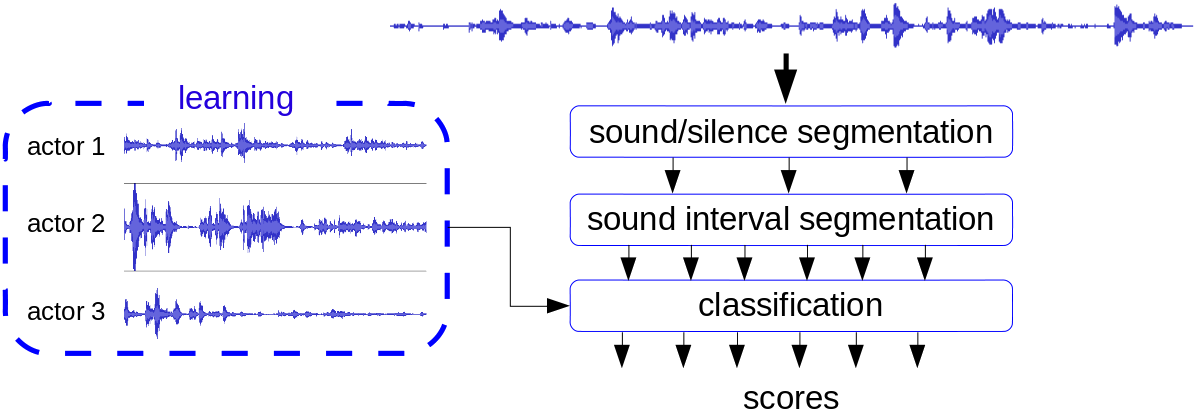
\includegraphics[width=\columnwidth]{diarizationT.png}
%\caption{In the speaker diarization phase, we learn a model of each actor's voice.
%They are used as observation probabilities in our Semi-Markov model of the rehearsals.}
%\label{fig_diarization}
%\end{figure}


\subsubsection{Actor detection and recognition} 

Based on their appearance model, we separately detect all actors present on stage. The qualitative results on this sequence 
are presented in Fig.~\ref{fig_tracking_coahtr}. This example is particularly challenging  because of the fast displacements 
of the actors and the frequent occlusions between actors. 

\begin{figure}[tp]
\centering
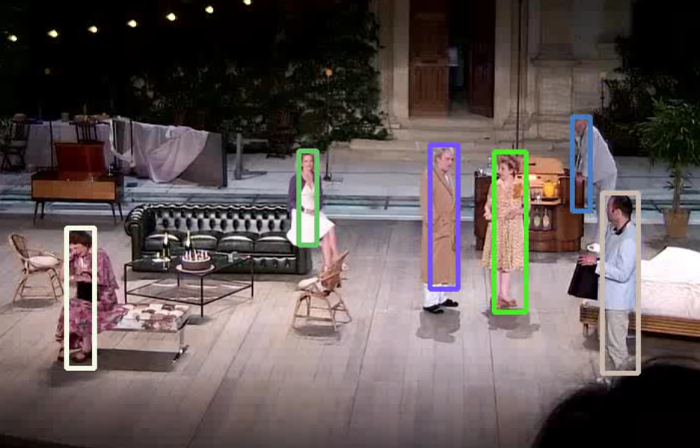
\includegraphics[width=\columnwidth]{tracking_coahtr}
\caption{Tracking of  the six characters of sequence $\mathcal{S}_4$. Using actors specific detections gives 
an additional advantage in resolving multiple actor tracking.}
\label{fig_tracking_coahtr}
\end{figure}

Despite the challenging environment, our method provides very good results for the tracking of the six actors, where generic state-of -the-art tracking methods quickly drifted away from the target  and were unstable both in presence of occlusion and fast movements. 


%\cite{Nummiaro2002,Ross2008}  \cite{Kwon2010,Babenko2009} also drifted away with heavy occlusions.  \cite{Wang2011} failed because of large appearence changes and occlusions. Only our algorithm maintains its performance in this challenging example.



\subsection{Applicative plateforme for data exposure}
Ligne de temps (nicolas , PA)

\subsubsection{Ingest}

\subsubsection{Search engine}

\subsubsection{Metadata player}

\subsection{Linked Open Data  publication}
Important : au service d'un digital heritage, implication de l'open data pour le patrimoine. (PA)



%%%%%%%%%%%%%%%%
\section{Archive Valorisation Scenarios}
\todo{(1,5 pages)}

\subsection{Visualization and browsing strategies}


\subsection{Demonstrator for Brick and Maggie scene}
For some selected scenes, we offer a fine-grained browsing interface allowing to zoom both temporally and spatially
thought the archive, by making use of the audio and video processing described in Section 4.  

\subsubsection{Temporal zoom}

\subsubsection{Spatial zoom}
The source video  is recorded from a distant viewpoint  to provide  a general  view of the stage.  None of what occurs in the stage is missing but the video is not pleasant to watch.  The theater performances are often edited like a movie to be more attractive.   It is easy to more precisely annotate the script of the play with some simple information as who speak to whom. With our method, we can temporally match the script to the video.  The positions of the characters in the frames are given by our tracking algorithm.  From there, by referring to usual editing rules, we can realize an automatic editing of the performance (Fig.~\ref{fig_speaker}) using methods described elsewhere \cite{Gandhi14}.  For example, during a monologue we realize an medium-shot of the speaker and during a dialogue we realize a two-shot that contains the speaker and his adresse. This greatly improves the visibility of the main actors, and makes it possible to focus on their gestures and facial expressions, as opposed to the general view, which is more useful to appreciate the choreography of their movements on stage.

\begin{figure*}[tp]
\centering
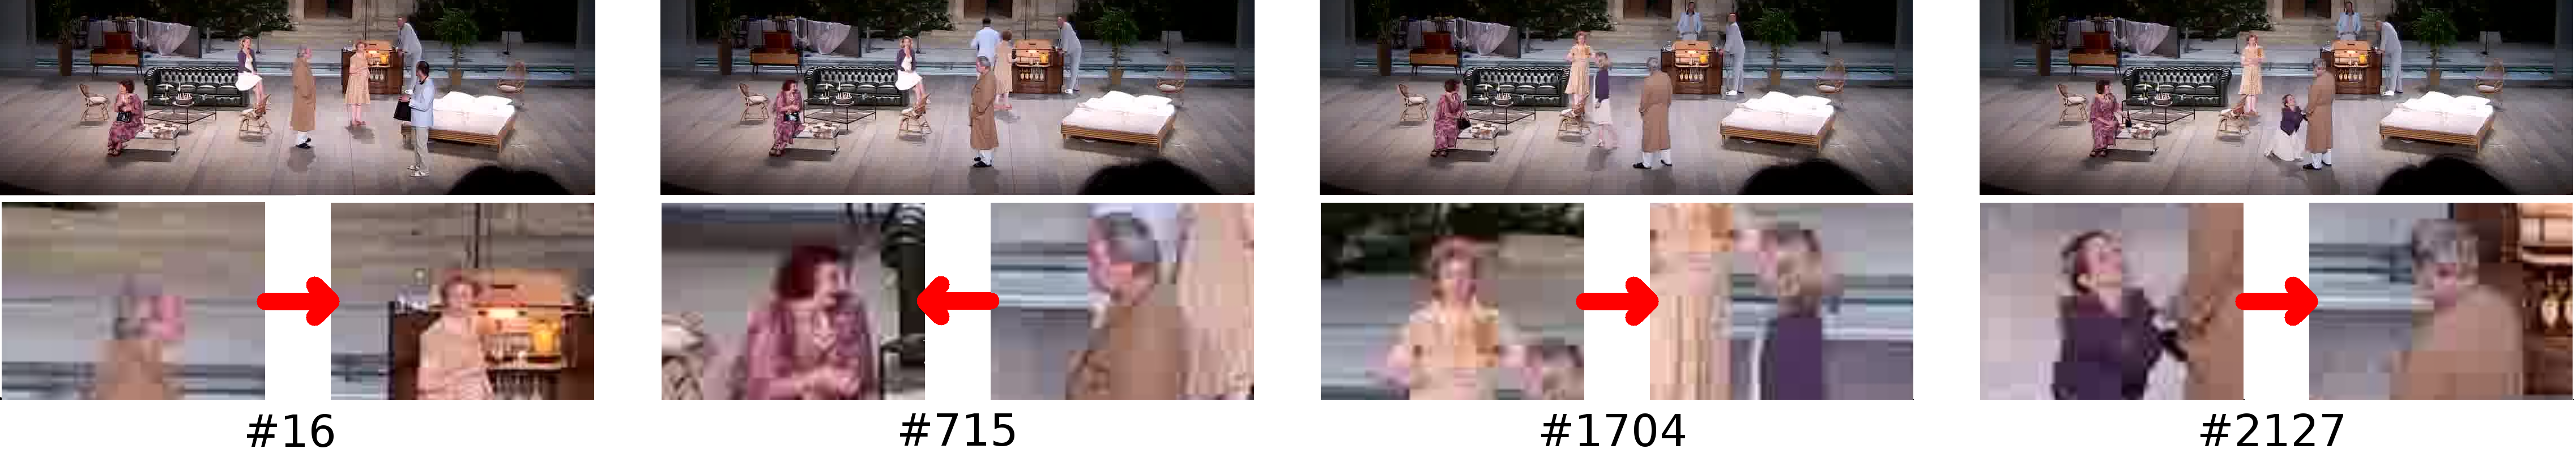
\includegraphics[width=\textwidth]{speakers2}
\caption{Reframing of the videos at the speaker and the interlocutor levels. Audio-to-text alignment temporally localizes the cues and the actors tracking spatially localizes the characters on the frames. 
This figure displays the automatic reframing process obtained for several frames on the sequence $\mathcal{S}_4$. The arrows go from the speaker to the interlocutor.}
\label{fig_speaker}
\end{figure*}


Future work is needed to fully evaluate this feature. We were inspired by the zoom-lens model of consciousness \cite{Eriksen86}, 
which proposes  that human perception  may in fact compose a movie from all available visual  stimuli  ; and by the theory 
of spectatorship, which surveys the audience's visuo-motor behavior  during a performance \cite{Bennett97}.   





\subsection{Mobile app} If space permits !

Maquettes ?

Not sure that this is relevant here !


\subsection{Experimental validation}
The recordings have been evaluated subjectively by the actors, the director and her assistants ?

A separate evaluation is being performed by film editors.

We can use Pascal Bouchez evaluation grids to assess the quality of the dataset ?


%%%%%%%%%%%%%%%%%%%%%%%%%%%
\section{Limitations and Future  Work}
\todo{(0.25 pages)}

Reframing and play text alignment is experimental and needs to be further validated and automated.

Better image resolution may be useful (4K, 8K).

Stereoscopic 3D images requires future work.

Reverse shots of the director and her assistances would be valuable.

Sound quality is a problem that can be addressed with better microphones.

More work is needed to extrapolate to other performances - concert, opera, ballet.

Graphical annotations would be useful.

Future work is needed for assigning the virtual cameras automatically.



%%%%%%%%%%%%%%%%%%%%%%%%%%%
\section{Conclusion}
\todo{(0.25 pages)}

Our technology is non intrusive and well accepted by the production team

It is made available to researchers in genetic analysis.




 
% conference papers do not normally have an appendix

% use section* for acknowledgement
\section*{Acknowledgment}

The authors would like to thank...





% trigger a \newpage just before the given reference
% number - used to balance the columns on the last page
% adjust value as needed - may need to be readjusted if
% the document is modified later
%\IEEEtriggeratref{8}
% The "triggered" command can be changed if desired:
%\IEEEtriggercmd{\enlargethispage{-5in}}

% references section
%\nocite{*}


% can use a bibliography generated by BibTeX as a .bbl file
% BibTeX documentation can be easily obtained at:
% http://www.ctan.org/tex-archive/biblio/bibtex/contrib/doc/
% The IEEEtran BibTeX style support page is at:
% http://www.michaelshell.org/tex/ieeetran/bibtex/
\bibliographystyle{IEEEtran}
% argument is your BibTeX string definitions and bibliography database(s)
\bibliography{rehearsals}



% that's all folks
\end{document}


